\let\negmedspace\undefined
\let\negthickspace\undefined
\documentclass[article]{IEEEtran}
\usepackage[a5paper, margin=10mm, onecolumn]{geometry}
\usepackage{tfrupee}

\setlength{\headheight}{1cm}
\setlength{\headsep}{0mm}

\usepackage{gvv-book}
\usepackage{gvv}
\usepackage{cite}
\usepackage{amsmath,amssymb,amsfonts,amsthm}
\usepackage{algorithmic}
\usepackage{graphicx}
\usepackage{textcomp}
\usepackage{xcolor}
\usepackage{txfonts}
\usepackage{listings}
\usepackage{enumitem}
\usepackage{mathtools}
\usepackage{gensymb}
\usepackage{comment}
\usepackage[breaklinks=true]{hyperref}
\usepackage{tkz-euclide} 
\usepackage{listings}                                       
\def\inputGnumericTable{}                                 
\usepackage[latin1]{inputenc}                                
\usepackage{color}                                            
\usepackage{array}                                            
\usepackage{longtable}                                       
\usepackage{calc}                                             
\usepackage{multirow}                                         
\usepackage{hhline}                                           
\usepackage{ifthen}                                           
\usepackage{lscape}

\renewcommand{\thefigure}{\theenumi}
\renewcommand{\thetable}{\theenumi}
\setlength{\intextsep}{10pt}

\numberwithin{figure}{enumi}
\renewcommand{\thetable}{\theenumi}
\begin{document}
\bibliographystyle{IEEEtran}
\title{NCERT-12.6.5.1.2}
\author{EE24BTECH11035 - KOTHAPALLI AKHIL}
{\let\newpage\relax\maketitle}
\noindent\textbf{Question: }  
Finding Minimum and Maximum Values of $y = 9x^2 + 12x + 6$.\\
\solution \\
\textbf{Theoretical Method:}\\
We aim to find the minimum and maximum values of the quadratic function $y = 9x^2 + 12x + 6$. First, we calculate the first derivative of $y$ with respect to $x$:

\begin{align}
\frac{dy}{dx} &= 18x + 12
\end{align}

Setting the derivative equal to zero, we find the critical points:

\begin{align}
18x + 12 &= 0 \\
x &= -\frac{2}{3}
\end{align}

To determine whether this critical point is a minimum or maximum, we compute the second derivative:

\begin{align}
\frac{d^2y}{dx^2} &= 18
\end{align}

Since $\frac{d^2y}{dx^2} > 0$, the function has a minimum at $x = -\frac{2}{3}$. Now, we calculate the corresponding $y$ value:

\begin{align}
y &= 9\left(-\frac{2}{3}\right)^2 + 12\left(-\frac{2}{3}\right) + 6 \\
&= 9 \times \frac{4}{9} - 8 + 6 \\
&= 4 - 8 + 6 \\
&= 2
\end{align}

Thus, the minimum value of $y$ is $2$ at $x = -\frac{2}{3}$. Since the parabola opens upwards, it has no maximum value as $x \to \infty$.

\textbf{Computational Method:}

In the computational method, we use an iterative approach, specifically gradient descent, to approximate the minimum of the function. The process involves the following steps:

\begin{itemize}
    \item \textbf{Initialization:} We start with an initial guess for $x$ (e.g., $x = 0$) and set parameters like the learning rate ($lr$) and a threshold for convergence ($\epsilon$).
    \item \textbf{Gradient Calculation:} The gradient of the function $y = 9x^2 + 12x + 6$ with respect to $x$ is given by $dy/dx = 18x + 12$.
    \item \textbf{Update Rule:} In each iteration, we update $x$ using the formula:
    \begin{align}
    x_{\text{new}} = x_{\text{old}} - lr \times \frac{dy}{dx}
    \end{align}
    \item \textbf{Convergence Check:} The iterations continue until the gradient magnitude is less than the threshold $\epsilon$, indicating that we are close to a minimum.
\end{itemize}

\noindent\textbf{Steps in the Algorithm:}

\begin{enumerate}
    \item Initialize $x = 0$, $lr = 0.01$, and $\epsilon = 10^{-6}$.
    \item Calculate the gradient $\frac{dy}{dx}$.
    \item Update $x$ using the update rule.
    \item Check if $|\frac{dy}{dx}| \leq \epsilon$. If true, stop; otherwise, repeat.
\end{enumerate}

\noindent\textbf{Advantages and Limitations:}
\begin{itemize}
    \item \textbf{Advantages:} Gradient descent is useful for finding minima in cases where analytical solutions are difficult or impossible. It provides an iterative way to approximate solutions.
    \item \textbf{Limitations:} The accuracy depends on the learning rate and the number of iterations. A poorly chosen learning rate can lead to slow convergence or divergence.
\end{itemize}
For the above Question,\\
The Theoritical value found is 2.\\
The Computational value found is 2.\\
Therefore,Using of gradient descent method is highly accurate depending upon its learning rate.
 \begin{figure}[h!]
	\centering
	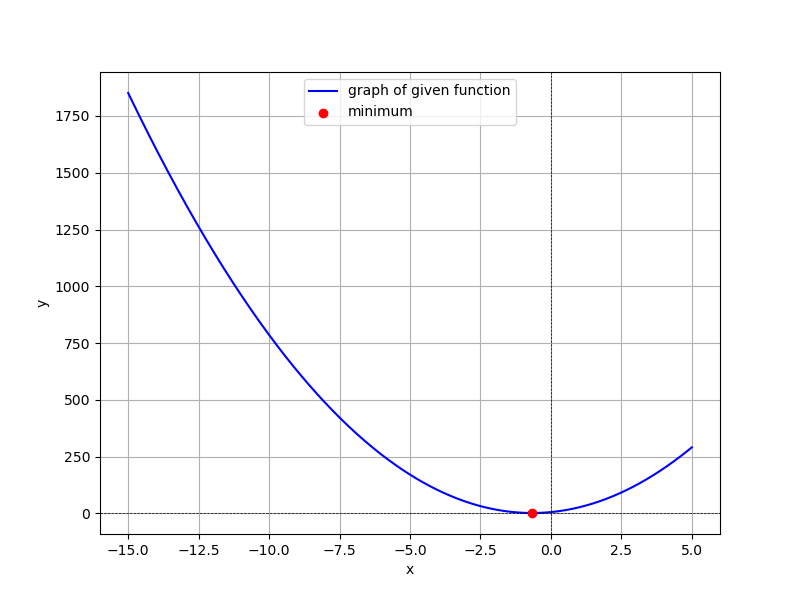
\includegraphics[width=\columnwidth]{figures/Figure_1.png}
	 \caption{Minimum value of the given function}
	\label{stemplot}
\end{figure}
\end{document}

